
%%%%%%%%%%%%%%%%%%%%%%%%%%%%%%%%%%%%%%%%%%%%%%%%%%%%%%%%%%%%%%%%%%%%%%%%%%%%%%%%%%%%%%%%%%%%%%%%
% Hydrostatik                                   
%%%%%%%%%%%%%%%%%%%%%%%%%%%%%%%%%%%%%%%%%%%%%%%%%%%%%%%%%%%%%%%%%%%%%%%%%%%%%%%%%%%%%%%%%%%%%%%%
\newpage
\section{Fluide}
	\subsection{Einführung}
	\subsubsection{Definitionen}
		\begin{minipage}{19cm}
			\begin{itemize}
				\item \textbf{ideale Flüssigkeit:}
					\begin{itemize}
						\item Reibungsfrei (nicht viskos)
						\item Inkompressibel
					\end{itemize}
			\end{itemize}
		\end{minipage}
	\newline
	\newline
	
	\subsubsection{Druck}
		\begin{minipage}[t]{13cm}
			\myparagraph{Definition}
				\renewcommand{\arraystretch}{2.5}
				\begin{tabular}{ p{4cm} | p{7cm}}
					$p = \dfrac{F_{\perp}}{A}$	&	$p$ = Druck in $\frac{N}{m^2}$ = $Pa$\\
					$\tau = \dfrac{F_{\parallel}}{A} $	& $\tau$ = Schubspannung in $\frac{N}{m^2}$\\
				\end{tabular}
				\renewcommand{\arraystretch}{1.5}
				\begin{tabular}{ p{4cm} | p{7cm} }
					& $F_{\perp}$ = senkrechte Kraftkomponente in $N$\\
					& $F_{\parallel}$ = parallele Kraftkomponente in $N$\\
					& $A$ = Fläche in $m^2$\\
				\end{tabular} 
				\renewcommand{\arraystretch}{1}
		\end{minipage}
		\begin{minipage}[t]{5cm}
			\vspace{-\ht\strutbox}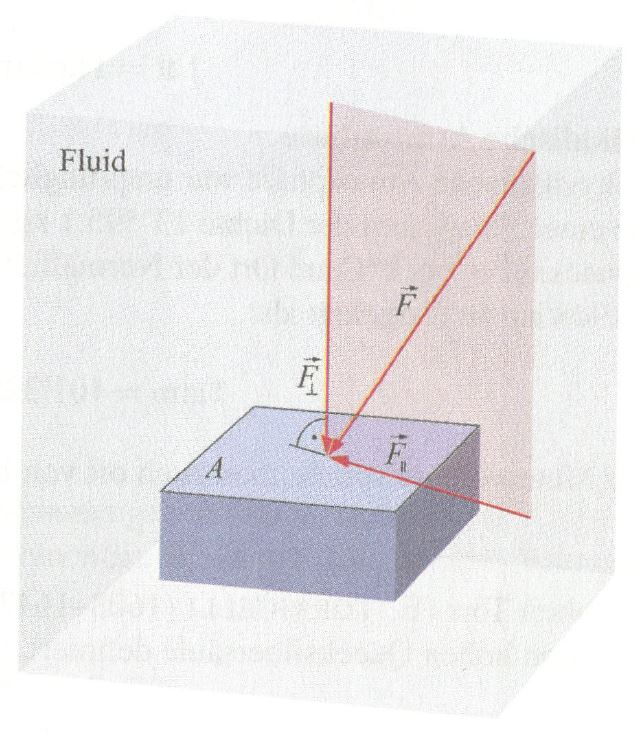
\includegraphics[width=4.5cm]{./bilder/Druck.jpg}
		\end{minipage}
		\newline
		\newline
		\begin{minipage}[t]{12cm}
			\myparagraph{Druckeinheiten}
				\renewcommand{\arraystretch}{1.5}
				\begin{tabular}{ p{4cm} | p{9cm}}
					1 bar = $10^5$ Pa\\
					1 at = $9.807 \cdot 10^4$ Pa	&	at = technische Atmosphäre\\
					1 atm = $1.013 \cdot 10^5$ Pa	&	atm = physikalische Atmosphäre\\
					1 Torr = 133.3 Pa	&	Torr = Millimeter Quecksilbersäule\\
					1 psi = $6.895 \cdot 10^3$ Pa	&	psi = angelsächsische Einheit (pound per square inch)\\
				\end{tabular}
				\renewcommand{\arraystretch}{1}
		\end{minipage}
		\newline
		\newline
		\newline
		\newline
		\begin{minipage}[t]{11.5cm}
			\myparagraph{Gesetz von Pascal}
				\newline
				Druck ist nicht Richtungsabhängig!\\ \\
				\renewcommand{\arraystretch}{1.5}
				\begin{tabular}{ p{4cm} | p{7cm}}
					$p_a = p_b = p_c$	&	$p_a$ = Druck auf Fläche $a \cdot h$\\
					&	$p_b$ = Druck auf Fläche $b \cdot h$\\
					&	$p_c$ = Druck auf Fläche $c\cdot h$\\
				\end{tabular}\\ \\ \\
		\end{minipage}
		\begin{minipage}[t]{10cm}
			\vspace{-\ht\strutbox}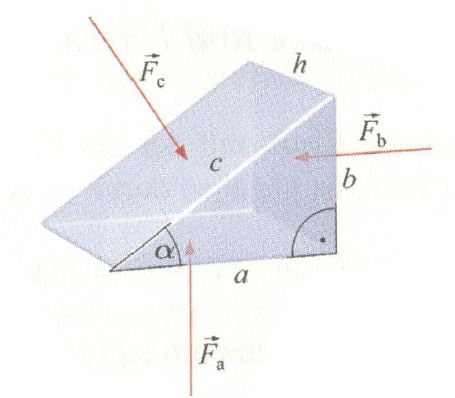
\includegraphics[width=5.5cm]{./bilder/GesetzVonPascal1.jpg}
			\vspace{-\ht\strutbox}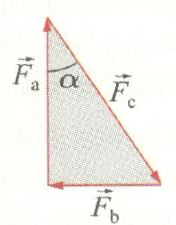
\includegraphics[width=2cm]{./bilder/GesetzVonPascal2.jpg}
		\end{minipage}
	\newpage
	\subsubsection{Kompression}
		\begin{minipage}[t]{13cm}
			\myparagraph{Kompressibilität}
				\renewcommand{\arraystretch}{2.5}
				\begin{tabular}{ p{4cm} | p{7cm}}
					$\kappa = -\dfrac{1}{V} \dfrac{\Delta V}{\Delta p}$	&	$\kappa$ = Kompressibilität in $\frac{1}{Pa}$\\
				\end{tabular}
				\renewcommand{\arraystretch}{1.5}
				\begin{tabular}{ p{4cm} | p{7cm} }
					& $V$ = Volumen in $m^2$\\
					& $p$ = Druck in $Pa$\\
				\end{tabular} 
				\renewcommand{\arraystretch}{1}
		\end{minipage}
		\newline
		\begin{minipage}[t]{13cm}
			\myparagraph{Kompressionsmodul}
			\renewcommand{\arraystretch}{2.5}
			\begin{tabular}{ p{4cm} | p{7cm}}
				$K = \dfrac{1}{\kappa} = -V \dfrac{\Delta p}{\Delta V}$	&	$\kappa$ = Kompressibilität in $\frac{1}{Pa}$\\
			\end{tabular}
			\renewcommand{\arraystretch}{1.5}
			\begin{tabular}{ p{4cm} | p{7cm} }
				& $K$ = Kompressionsmodul in $Pa$\\
				& $V$ = Volumen in $m^2$\\
				& $p$ = Druck in $Pa$\\
			\end{tabular} 
			\renewcommand{\arraystretch}{1}
		\end{minipage}

\newpage	
\subsection{Hydrostatik}
	\subsubsection{Schweredruck}
		\begin{minipage}[t]{13cm}
			\myparagraph{Flüssigkeiten}
				\begin{flushleft}
					Hydrostatisches Paradoxon: Der Schweredruck in einer ruhenden Flüssigkeit ist nur von der Höhe in der Flüssigkeit, nicht aber von der Form des Gefässes abhängig.
				\end{flushleft}
				\renewcommand{\arraystretch}{1.5}
				\begin{tabular}{ p{4cm} | p{7cm}}
					$p = \rho gh$	&	$p$ = Druck in $Pa$\\
					& $\rho$ = Dichte in $\frac{kg}{m^3}$\\
					& $g$ = Gravitationsfeldstärke = $9.81\frac{m}{s^2}$\\
					& $h$ = Höhe in $m$ (unter Wasseroberfläche)\\
				\end{tabular}
				\renewcommand{\arraystretch}{1}
		\end{minipage}
		\begin{minipage}[t]{10cm}
			\vspace{-\ht\strutbox}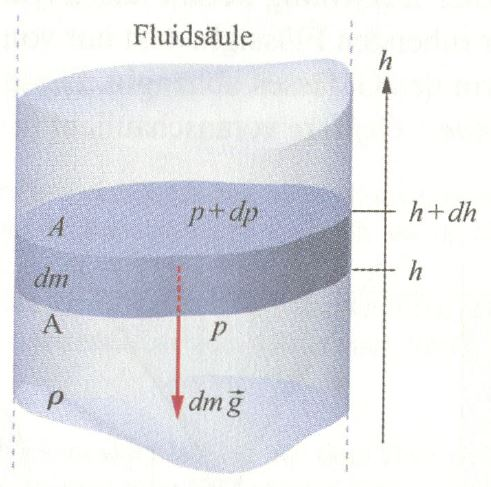
\includegraphics[width=5cm]{./bilder/Schweredruck.jpg}
		\end{minipage}
		\newline
		\newline
		\newline
		\begin{minipage}[t]{13cm}
			\myparagraph{Gase (Barometrische Höhenformel für isotherme Atmosphäre)}
			\renewcommand{\arraystretch}{1.5}
			\begin{tabular}{ p{4cm} | p{7cm}}
				$p = p_0 e^{-\frac{\rho_0}{p_0}gh}$	&	$p$ = Druck in $Pa$\\
				& $\rho$ = Dichte in $\frac{kg}{m^3}$\\
				& $g$ = Gravitationsfeldstärke = $9.81\frac{m}{s^2}$\\
				& $h$ = Höhe in $m$\\
			\end{tabular}
			\renewcommand{\arraystretch}{1}
		\end{minipage}
	
	\subsubsection{Statischer Auftrieb (Archimedisches Prinzip)}
		\begin{minipage}[t]{13cm}
			Der Auftrieb eines in ein Fluid eingetauchten Körpers ist gleich dem Gewicht des von ihm verdrängten Fluids.\\
			Der Auftrieb ist unabhängig von der Tiefe!\\ \\
			\renewcommand{\arraystretch}{1.5}
			\begin{tabular}{ p{4cm} | p{7cm}}
				$F_A = F_G$	&	$F_A$ = Auftriebskraft in $N$\\
				$F_A = \rho_{fl} \cdot g \cdot V_{fl}$	& $F_G$ = Gewichtskraft in $N$\\
				$F_G = m_K \cdot g = \rho_k \cdot g \cdot V_K$	& $\rho_{fl}$ = Dichte des Fluids in $\frac{kg}{m^3}$\\
				& $\rho_{k}$ = Dichte des Festkörpers in $\frac{kg}{m^3}$\\
				& $V_{fl}$ = Von Festkörper verdrängtes Fluid-Volumen in $m^3$\\
				& $m_K$ = Masse Festkörper in $kg$\\
				& $V_K$ = Volumen Festkörper in $m^3$\\
			\end{tabular}
			\renewcommand{\arraystretch}{1}
		\end{minipage}
		\begin{minipage}[t]{10cm}
			\vspace{-\ht\strutbox}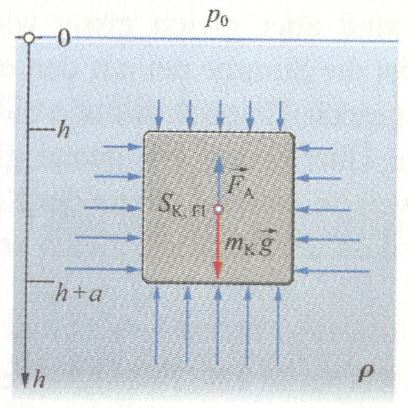
\includegraphics[width=5cm]{./bilder/StatischerAuftrieb.jpg}
		\end{minipage}
	
	\subsubsection{Grenzflächeneffekte}
		\begin{minipage}[t]{10.5cm}
			\myparagraph{Oberflächenspannung, spez. Oberflächenenergie (Van der Waals-Kraft)}
			\newline
			Kräfte zwischen Atomen oder Molekülen an der Oberfläche eines Fluides.\\ \\
			\renewcommand{\arraystretch}{2.5}
			\begin{tabular}{ p{4cm} | p{7cm}}
				$\sigma = \dfrac{F}{l} = \dfrac{\Delta W}{\Delta A}$	&	$\sigma$ = Oberflächenspannung in $\frac{N}{m}$\\
			\end{tabular}
			\renewcommand{\arraystretch}{1}
		\end{minipage}
		\begin{minipage}[t]{10cm}
			\vspace{-\ht\strutbox}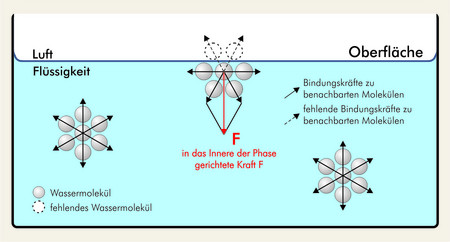
\includegraphics[width=8cm]{./bilder/VanDerWaalsKraft.jpg}
		\end{minipage}
		\newline
		\newline
		\newline
		\begin{minipage}[t]{12cm}
			\myparagraph{Grenzflächenspannung}
			\renewcommand{\arraystretch}{2.5}
			\begin{tabular}{ p{4cm} | p{7cm}}
				$cos(\varphi) = \dfrac{\sigma_{sg}-\sigma_{sl}}{\sigma_{lg}}$	&	$\varphi$ = Kontaktwinkel in rad\\
			\end{tabular}
			\renewcommand{\arraystretch}{1.5}
			\begin{tabular}{ p{4cm} | p{7cm}}
				& $\sigma_{sl}$ = Grenzflächenspannung zw. Festkörper und Flüssigkeit in $\frac{N}{m}$\\
				& $\sigma_{sg}$ = Grenzflächenspannung zw. Festkörper und Gas in $\frac{N}{m}$\\
				& $\sigma_{lg}$ = Grenzflächenspannung zw. Flüssigkeit und Gas in $\frac{N}{m}$\\
			\end{tabular}
			\renewcommand{\arraystretch}{1}
		\end{minipage}
		\begin{minipage}[t]{10cm}
			\vspace{-\ht\strutbox}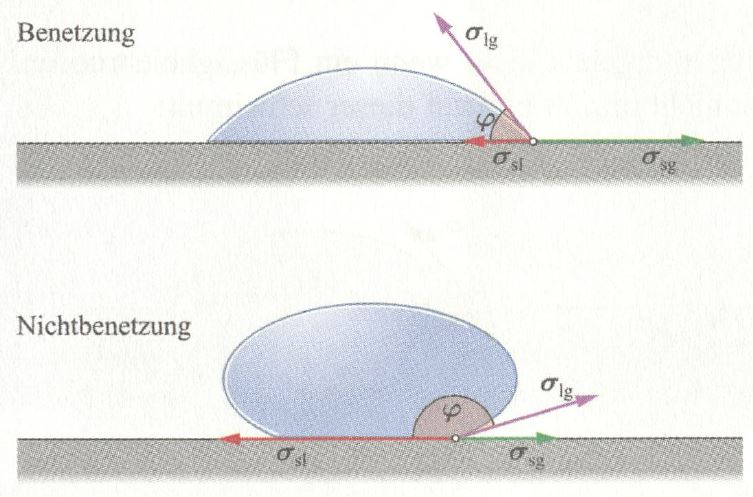
\includegraphics[width=7cm]{./bilder/Grenzflaechenspannung.jpg}
		\end{minipage}
		\newline
		\newline
		\newline
		\begin{minipage}[t]{12cm}
			\myparagraph{Kapillarität}
				\renewcommand{\arraystretch}{2.5}
				\begin{tabular}{ p{4cm} | p{7cm}}
					$h = \dfrac{2 \sigma}{\rho gr}$	&	$\sigma$ = Oberflächenspannung in $\frac{N}{m}$\\
				\end{tabular}
				\renewcommand{\arraystretch}{1.5}
				\begin{tabular}{ p{4cm} | p{7cm}}
					& $h$ = Steighöhe in m\\
					& $\rho$ = Dichte Flüssigkeit in $\frac{kg}{m^3}$\\
					& $r$ = Radius des Röhrchens in $m$\\
				\end{tabular}
				\renewcommand{\arraystretch}{1}
		\end{minipage}
		\begin{minipage}[t]{10cm}
			\vspace{-\ht\strutbox}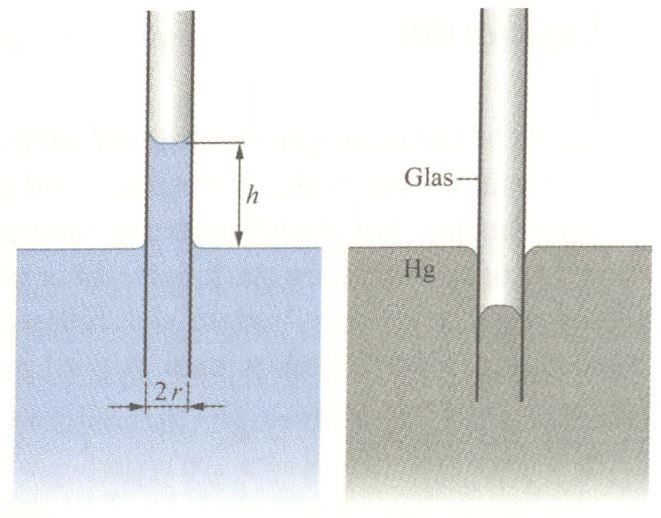
\includegraphics[width=7cm]{./bilder/Kapillaritaet.jpg}
		\end{minipage}
	